\documentclass[UTF8,a4paper]{ctexart}
\usepackage[utf8]{inputenc}
\usepackage{amsmath}
\usepackage{pdfpages}
\usepackage{graphicx}
\usepackage{wrapfig}
\usepackage{listings}
\usepackage{multicol}
\newcommand{\tabincell}[2]{\begin{tabular}{@{}#1@{}}#2\end{tabular}}
\title{智能交通仿真平台程序说明}
\author{张蔚桐\ 2015011493\ 自55}
\begin {document}
\maketitle
\clearpage
\section{程序架构}
\begin{figure}
\centering
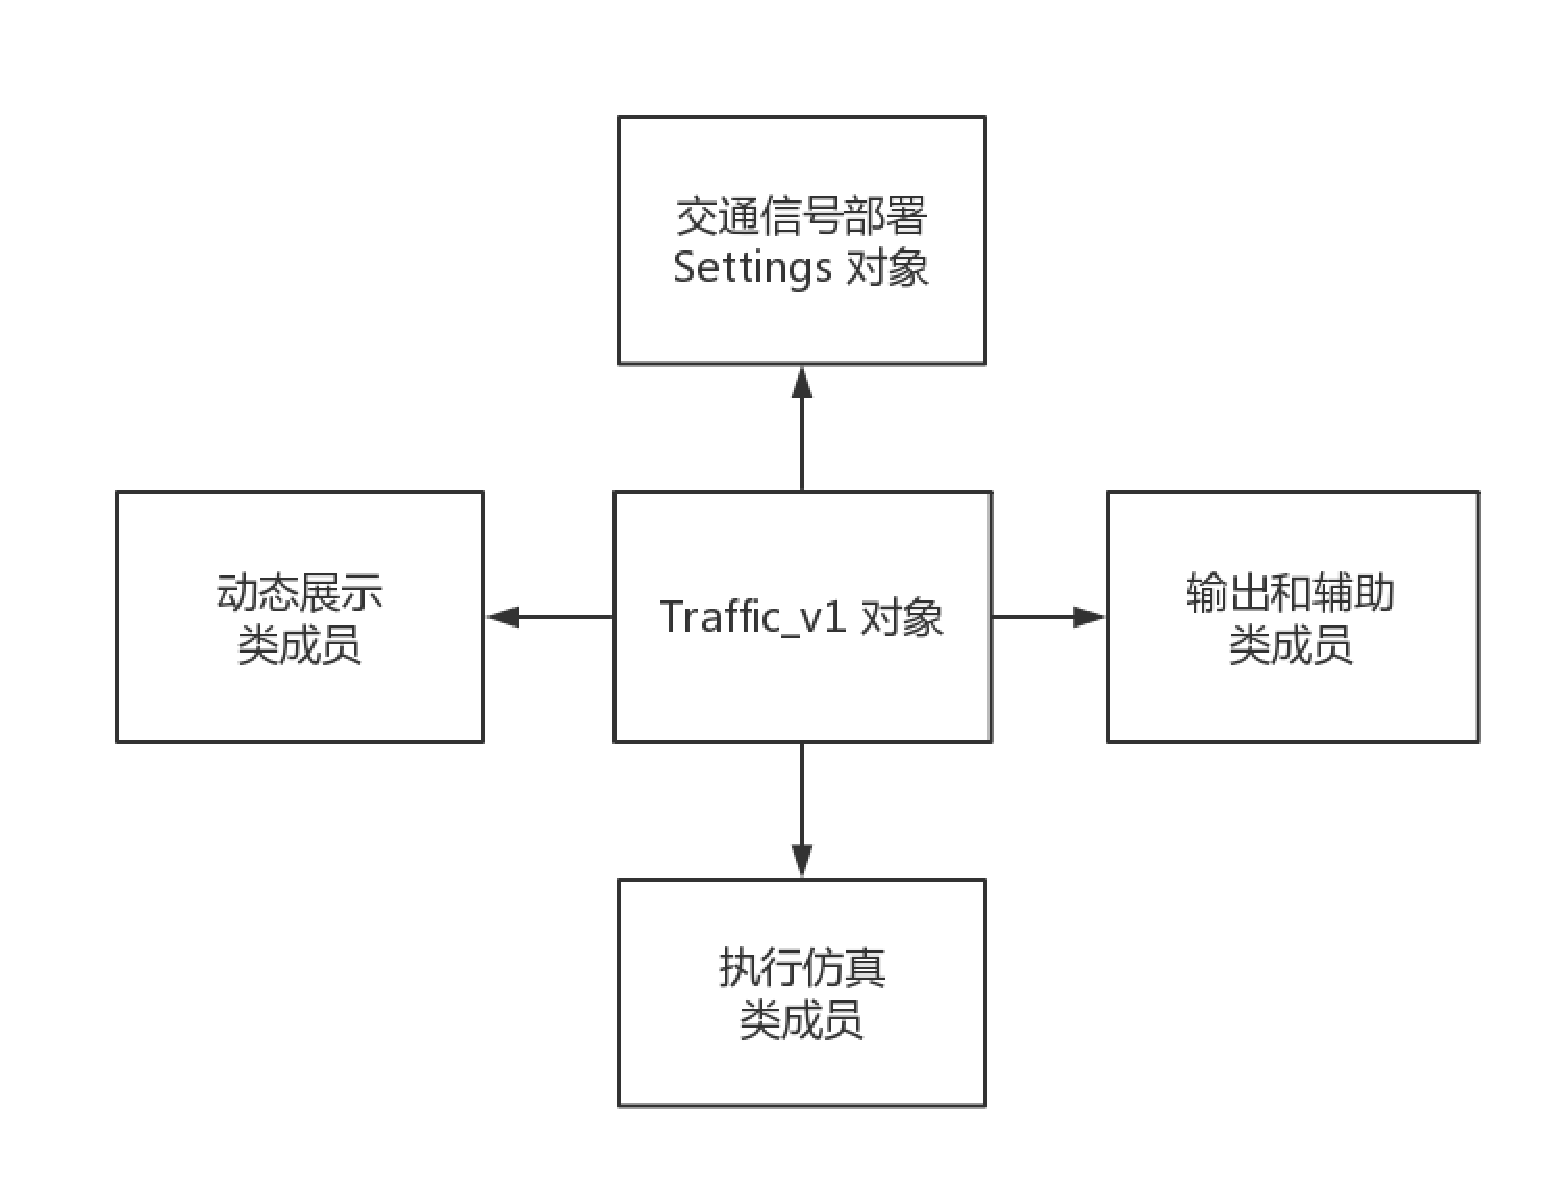
\includegraphics[width=\textwidth]{ClassDiagram.eps}
\caption{主体程序架构}
\label{Trafficv1}
\end{figure}
整个程序使用C++/Qt进行开发,核心由一个Traffic\_v1对象构成,这个对象的UML图如图(\ref{Trafficv1})所示

其中大致可以分为以下几个模块
\clearpage
\subsection{显示模块}
这些类成员主要为用户界面显示和调整设计,其中包括
\begin{multicols}{2}
\begin{lstlisting}[language=C++]
QPushButton* end;
QPushButton* edit;
QRadioButton* fast;
QRadioButton* medium;
QRadioButton* slow;
QRadioButton* very_slow;
QLabel* speed;
QLabel* ratio;
QSlider* ratio_setting;
QLabel* ratio_shower;
com_label* st;
com_label* _st;
QSlider* A_L;
QSlider* B_L;
QSlider* C_L;
QSlider* D_L;
QLabel*A_A;
QLabel*B_A;
QLabel*C_A;
QLabel*D_A;
QLabel*A_B;
QLabel*B_B;
QLabel*C_B;
QLabel*D_B;
\end{lstlisting}
停止按钮 \\
信号部署编辑 \\
快速(1000倍速) \\
中速(100倍速) \\
低速(10倍速) \\
极低速(1倍速)(仅用于debug) \\
“speed”标签\\
“Ratio Controled”标签\\
设置控制车辆比例的滑动条\\
显示控制车辆比例的标签\\
统计信息的类别的显示栏(12个)\\
统计信息的数据显示栏(12个)\\
设置车流量的滑块(W方向)\\
设置车流量的滑块(S方向)\\
设置车流量的滑块(E方向)\\
设置车流量的滑块(N方向)\\
W方向标签\\
S方向标签\\
E方向标签\\
N方向标签\\
W方向车流量数值显示\\
S方向车流量数值显示\\
E方向车流量数值显示\\
N方向车流量数值显示\\
\end{multicols}

程序每向前执行一步仿真就进行一次显示上的刷新,并将其绘制在左侧的交通信号口中,具体的实现见"paint.cpp",整个函数完成如下步骤
\begin{enumerate}
\item 绘制十字路口基本单元
\subitem 根据信号配时的部署绘制红绿灯
\subitem 绘制交通路口车道线
交通线显示长度为30m,宽度为当前标准宽度(六车道22.5m)
\item 绘制来车和离开的车辆

其中,开往交通路口的车辆可以接受控制,而驶出交通路口的车辆程序认为他们已经不必接受控制,并为他们自行补足了相关驾驶策略
\item 绘制交通路口内轨迹线

程序中没有处理车辆在交通路口内的行为,因此采用轨迹线代替车辆的具体位置。其中,当车辆进入交通路口后,我们认为左转,直行,右转车辆驶离交通路口的时间分别为3s,2s和1s,这些参数可以在simulate函数中进行相关的修改。而相应的轨迹线将持续对应的时间

可以认为,轨迹线的交叉次数是交通路口内混乱程度的表述,如果存在着过多的交叉次数,可能会影响交通路口的通行效率以及造成危险,但这主要是信号配时的问题
\end{enumerate}
\subsection{仿真模块}
这是程序执行的核心模块,按照前文仿真速度设置控件设置的仿真速度(快,中,慢以及极慢)提供一个间隔为1ms,10ms,100ms以及1000ms的触发信号QTimer*timer;

接受触发信号之后,程序按照如图(\ref{timeflow})执行相关的操作

在执行流程中,进程控制块决定是否自动停止仿真(根据是否满足用户的停止仿真条件等),新车辆生成在每条车道上按照设计的算法生成车辆,用户策略配置将用户策略应用到即将驶入交通岗的每一台车辆上,而系统策略负责处理驶出交通岗的车辆以及某些处于边际情况的车辆。以上的策略,主要改变的是车辆的加速度,接下来的运动学仿真,根据车辆的加速度和速度,决定车辆下一个时刻的位置和速度。最终处理已经驶入交通路口或者即将完全驶出关心的范围的车辆。最终完成系统界面的重绘工作,并等待下一个触发信号的到来。

根据目前程序的执行情况,在100倍速(10ms)下,系统的负担是比较合适的,同时仿真数据也比较稳定,在1000倍速情况下可能出现一些时序上的问题
\begin{figure}
\centering
\includegraphics[width=\textwidth]{TimeFlow.png}
\caption{控制流程}
\label{timeflow}
\end{figure}
\subsection{输出和辅助模块}
这部分模块的主要工作在于将实时的仿真结果输出,其中的一部分在仿真过程图(\ref{timeflow})中,在系统重绘时调用,一部分随着仿真的进行,出现相关情况的边际执行。

随着仿真的进行,系统会建立四张csv表,存储在可执行文件(.exe)目录的根目录下的result文件夹中,result文件夹中的每一个文件夹的命名规则为

\centerline{\textbf{"具体日期+具体时间+仿真模式选择"}}

其中仿真模式选择的具体值将在后文算法设计中提到

四张表分别记录了不同类型的数据
\begin{enumerate}
\item car.csv

这张表记录了每辆车的初始速度(init\_velocity),理想到达时间(thoritical\_time),实际到达时间(act\_time)以及后两者的差值(delta),其中,理想到达时间表示为车辆以初始速度以最大加速度加速到最大限速,之后保持匀速直线运动状态直到驶入交通路口内部所花费的时间,实际时间是车辆经过这段路程实际花费的时间,他们的差值可以理解为车辆在路上浪费的时间
\item stop.csv

这张表记录了每个时刻每个车道停车的总数和系统内停车的总次数,以及占总车辆数的比例。

\item road.csv

这张表记录了每个时刻驶出某条车道的车辆总数和离开系统的车辆总数,以及他们的平均值
\item stop\_time.csv

这张表记录了每个时刻每个车道停车的总时间和系统内停车的总时间,以及分摊到每个车辆上的停车时间。
\end{enumerate}

一般来说,road.csv用来观测整个仿真过程是否正常,而剩余三张表用来评价整个策略的优劣

其中,停车次数按照车辆的速度低于某一设定阈值来确定,停车时间随着车辆的停车不断累加,而停车次数不随车辆的长期停车而改变

\subsection{交通灯设置模块}

交通灯设置模块完成自主定义交通灯的用户需求,其中三个按键“set red/green/yellow behind”完成的是对黑色时间线后面所有时间的选中的信号的设定。同时,此界面可以完成周期的设定,通过移动时间线或指定时间线位置,反复选中要更改的车道,设置信号相位等方式,可以完成没有限制的对周期执行的红绿灯信号的设置。同时,左侧界面会提示当前(黑色时间线时刻)可能栽 交通路口中出现的轨迹线,提示用户尽可能避免轨迹线的交叉等问题,帮助用户进行更合理的信号配时工作
\section{算法简述}
\subsection{程序基本参数和假定}
\subsection{车辆生成算法}
\subsection{跟驰策略的实现}
\subsection{无车路协同的自主策略的实现}
\subsection{有车路协同的自主策略的实现}
\subsection{混合驾驶的策略实现}
\section{运行结果}
\end{document}
